\documentclass[12pt]{article}
\usepackage{graphicx}
\usepackage{graphics}
\usepackage{refstyle}
\usepackage{amsmath}
\usepackage{caption}
\usepackage{float}
\usepackage{physics}
\usepackage{tasks}
\usepackage{listings}
\usepackage[utf8]{inputenc}
\graphicspath{{storage/self/primary/Download/maths/figs}}
\begin{document}
\begin{center}
	\section*{\textbf{Class 12}}
	\subsection*{Chapter 10 - Vector Algebra}
\end{center}
This is question 18 from exercise 10.5 \\
\begin{enumerate}
\item  The value of  $\hat{i} \cdot (\hat{j} \times \hat{k})$  + $\hat{j} \cdot (\hat{i} \times \hat{k})$ + $\hat{k} \cdot (\hat{i} \times \hat{j} )$ is
	\begin{tasks}(4)
    \task $0$ 
    \task $-1$ 
    \task $1$ 
    \task $3$  
\end{tasks}
\end{enumerate}
\textbf{Solution:}
\[
\begin{aligned}
\begin{tabular} {l|l}
$\hat{i} \times \hat{j} = \hat{k}$ &$\hat{j} \times \hat{i} = -\hat{k}$ \\
$\hat{j} \times \hat{k} = \hat{i}$ & $\hat{k} \times \hat{j} = -\hat{i}$ \\
$\hat{k} \times \hat{i} = \hat{j}$ &$\hat{i} \times \hat{k} = -\hat{j}$ \\
\end{tabular}
\end{aligned}
\]

Now,\\
\begin{center} 
$\hat{i} \cdot (\hat{j} \times \hat{k})$  + $\hat{j} \cdot (\hat{i} \times \hat{k})$ + $\hat{k} \cdot (\hat{i} \times \hat{j} )$ \\
= $\hat{i} \cdot (\hat{i}) + \hat{j} \cdot (-\hat{j}) + \hat{k} \cdot (\hat{k})$ \\
= $\hat{i} \cdot \hat{i} - \hat{j} \cdot \hat{j} + \hat{k} \cdot \hat{k}$ \\
\end{center}

\fbox{\begin{minipage}{15em}
$\hat{i} \cdot \hat{i} = |\hat{i}| |\hat{i}| \cos{0} $ \\
                       = $ 1 \times 1 \times 1 $ \\
                       = $ 1 $ \\
similarly, $ \hat{j} \cdot \hat{j} = \hat{k} \cdot \hat{k} = 1$
\end{minipage}}

\begin{center}
    = $ 1 - 1 + 1 $\\
    =$1$\\
\end{center}
So, option (c) is correct.

\begin{figure}[H]
	       \centering
		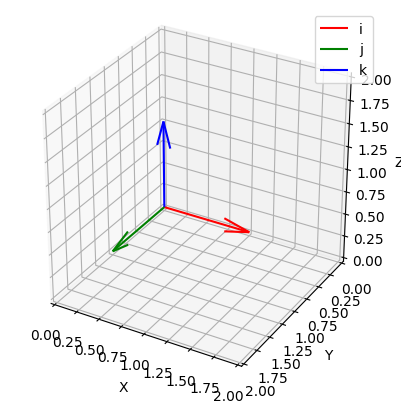
\includegraphics[width=\columnwidth]{figs/unit_vec.png}
                \label{fig:12/10/5/18}
	        \caption{fig:1}
               \end{figure}
\end{document}
